%%%%%%%%%%%%%%%%%%%%%%%%%%%%%%%%%%%%%%%%%%%%%%%%%%%%%%%%%%%%%%%
%
% Welcome to Overleaf --- just edit your LaTeX on the left,
% and we'll compile it for you on the right. If you open the
% 'Share' menu, you can invite other users to edit at the same
% time. See www.overleaf.com/learn for more info. Enjoy!
%
%%%%%%%%%%%%%%%%%%%%%%%%%%%%%%%%%%%%%%%%%%%%%%%%%%%%%%%%%%%%%%%
\documentclass[12pt, letterpaper]{article}
\usepackage{graphicx}
\usepackage{lipsum}
\usepackage{float}
\usepackage{array}

\title{Dual-shaft Electric Pump-fed Rocket Engine Design Review}
\author{Cooper Grau-Firkus}
\date{September 2024}

\begin{document}
\maketitle
\tableofcontents

\section{Introduction and Project Goals}

Potentially the most revolutionary development in the space industry in recent times has been the increasing access to spaceflight technologies by a greater number of people. This democratization of space technology has increased the rate of development by opening up to a much larger group of people. Part of this trend is the takeover of launch operations, in-space mobility, and mission operations by private industry. However, another major factor is the democratization of space technology and know-how not just to well-funded space industry startups, but also to students and hobbyists who have been able to take on ever more ambitious projects that would have been deemed near-impossible not very long ago. Twenty years ago, the first amateur rocket reached space, launched by the Civilian Space Exploration Team. Five years ago, the first student-built rocket to reach space, USC RPL's Traveler IV, crossed the Kármán line and reached speeds of over Mach 5. This year, the Gruyère Space Program student group demonstrated the first student-built Vertical Takeoff, Vertical Landing (VTVL) vehicle, called Colibri, and have carried out a rapid testing program of dozens of flights in only a few months. These incredible achievements and numerous others demonstrate that the standard ways of viewing space technology, as an inaccessible, expensive, and risky field of endeavor that can only be pushed forward by government or gargantuan companies may not be standard for much longer.

\begin{figure}[!b]
    \centering
    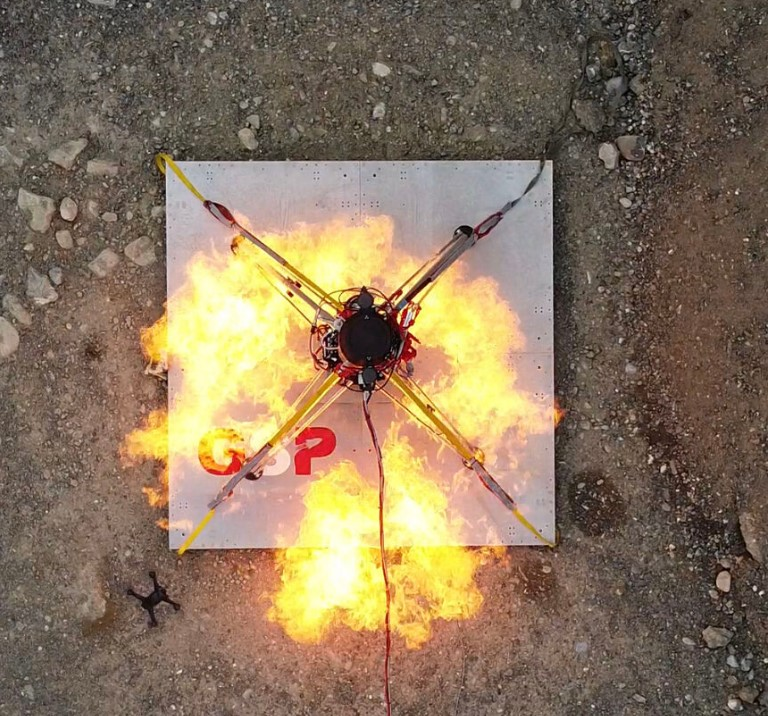
\includegraphics[width=7cm]{Images/Colibri.jpg}
    \caption{Gruyère Space Program's Colibri VTVL Testbed}
\end{figure}

\begin{figure}
    \centering
    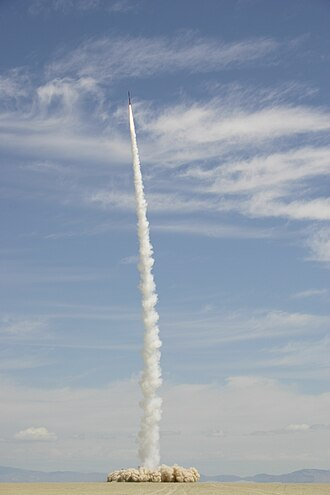
\includegraphics[width=5cm]{Images/Kluft-photo-CSXT-2004-amateur-space-launch.jpg}
    \caption{USC RPL Traveler IV Launch to Space}
\end{figure}

    
\newpage

This expansion of grassroots innovation in the space industry is a shift that has the potential to change the way that spaceflight technology is developed. Oftentimes, it is those who are considered outsiders in a field who are able to approach it from a new perspective and make the most impactful advancements. As more people gain access to space technology, more ideas will be not only generated, but also tested and sometimes proven. Our ability to move to and through space will expand in a positive feedback cycle in which the technologies and guidance developed by the people pushing the field forward today will lead to even more people able to push the field forward tomorrow. If we're lucky, this will result in a space industry that mirrors other industries with huge bases of support from hobbyists. Maybe one day soon, individuals will be able to go out and build or modify a high-power rocket, a VTVL craft, or a spacecraft the same way automotive hobbyists do today with their cars.

However, an area in which many of the most prominent technologies used in government and industry have not become available to students and hobbyists is the realm of liquid rocket propulsion. While the number of individuals and student groups who have hotfired an engine or even flown a liquid-fueled vehicle has seemed to increase rapidly, nearly all of these engines have been limited to a single class: the pressure-fed engine. While pressure-fed engines can teach many of the fundamental lessons of liquid propulsion, they omit the essential turbomachinery used to achieve high performance and thrust-to-weight ratio by just about every launch vehicle, and by many in-space vehicles and landers as well. An analysis of pressure-fed vs. pump-fed designs will be presented in the next section along with an attempt to explain why most student and hobbyist rockets have been pressure-fed designs up to this point.

The purpose of this document is to lay out in detail the process of creating a relatively small electric pump-fed liquid rocket engine, which I believe to be a good architecture for a first step toward engines which use turbomachinery. It is meant to serve as a guidebook and learning resource to those who may be interested in learning about these kinds of engines or in building one themselves. My hope is that this could serve as an effective and approachable enough resource to help encourage others to delve beyond pressure-fed engines and have some small part in spurring the positive feedback cycle of space technology development.

In addition, this document is meant to be a resource for design reviews of my electric pump-fed rocket engine and as a way for me to receive as much feedback as possible before lighting anything on fire. My goal for this project is to learn as much as possible about liquid propulsion technology and to grow as an amateur propulsion engineer. I hope that by open sourcing the majority of my work, I will be able to share my work more and receive more feedback than I otherwise would have. As I have made my way through the initial phases of my engine project, I have also found that it can often be very helpful to lay out my own thought and design processes as if I am presenting them to someone. This oftentimes exposes my own mistakes and leads to greater clarity.

\subsection{Pump-fed vs. Pressure-fed}

To understand why it is so important to gain experience with pump-fed engines, an analysis of the performance and operational differences between pump-fed and pressure-fed designs in pertinent. This analysis will also help to describe the fundamental differences, identify the reasons that amateur propulsion engineers have so far shied away from pump-fed engines, and will inform later analysis in this document of pump-fed vs. pressure-fed engines for specific flight vehicle designs.

While pressure-fed engines can also include simple thrusters, such as cold gas thrusters which use only propellant kinetic energy imparted via pressure and monopropellant thrusters that flow reactive propellants over a catalyst to create additional pressure and heat for thrust generation, here we are focused on bipropellant pressure-fed systems that are most comparable to pump-fed systems.

A likely reason why students and hobbyists most often choose to build pressure-fed systems is also one of the primary reasons they are used in the first place: mechanical simplicity, and the corresponding lower cost and developmental work required. In its most fundamental form, the only components that you need for a pressure-fed engine are:
\begin{itemize}
    \item Something to hold your propellants and pressurant, which is done by the tanks.
    \item Devices to control when your propellants flow, and how much, if needed. This is the job of the valves.
    \item Devices for combustion and thrust generation, primarily, the injector and thrust chamber.
\end{itemize}

These components can often be bought off-the-shelf, with the exception of the thrust chamber and injector. Compare this to a pump-fed design, which will require turbomachinery which must be specifically sized and meticulously tested for the given parameters of an engine, an often lengthy and costly process due to the necessity of hardware-rich testing which often includes testing to failure, leading to the destruction of early component iterations. Additionally, the added components of a pump-fed design will increase the weight of the engine in comparison to a pressure-fed design. This means that for identical vehicles powered by pressure-fed and pump-fed engines of equal and sufficiently low performance, the pressure-fed vehicle may actually achieve better performance due to a higher thrust to weight ratio.

\begin{figure}[t]
    \centering
    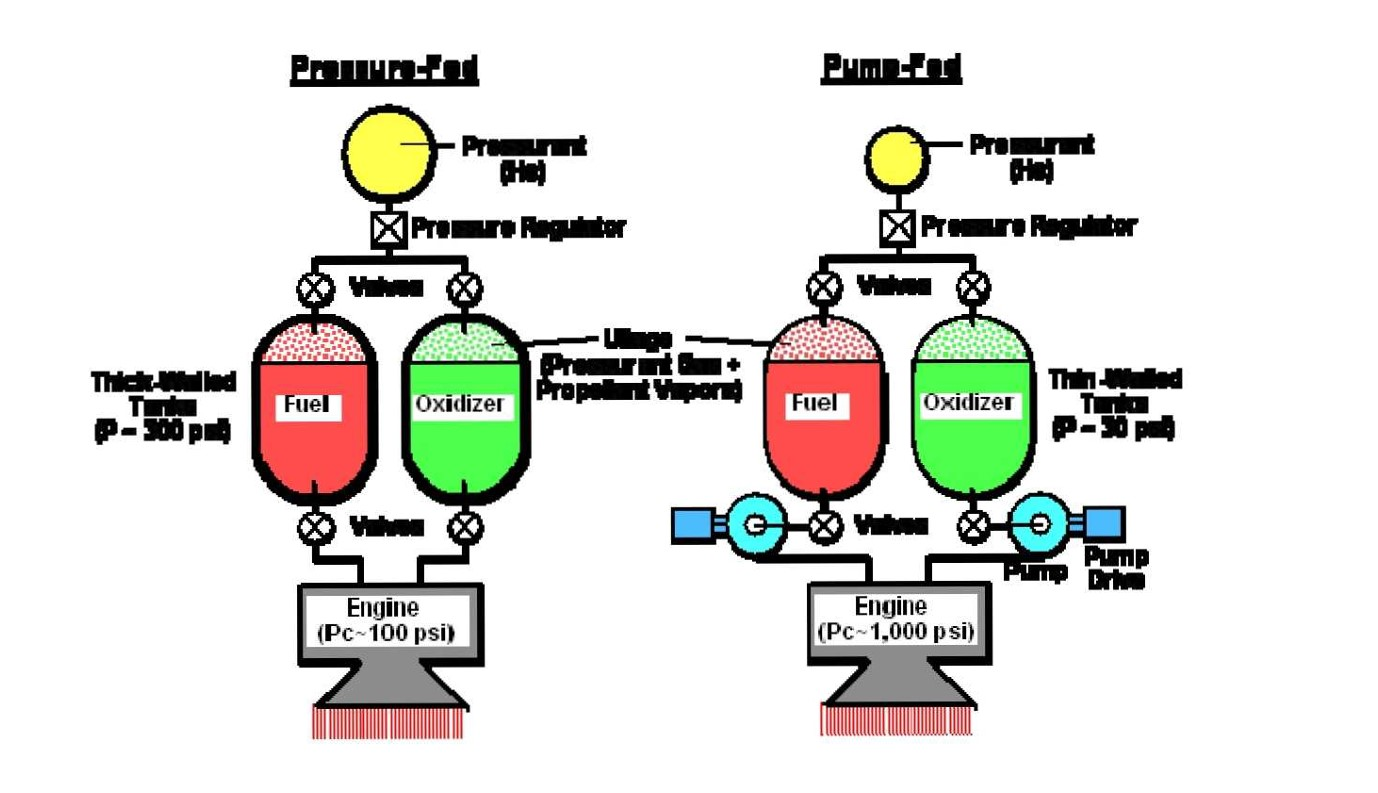
\includegraphics[width=15cm]{Diagrams/PumpVPressure.jpg}
    \caption{Simplified Schematics of Pressure-fed and Pump-fed Rocket Engines}
\end{figure}

\newpage

\begin{figure}[!t]
    \centering
    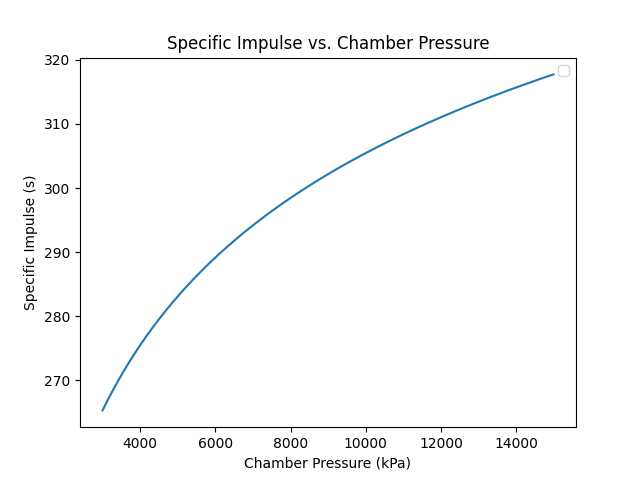
\includegraphics[width=8cm]{Plots and Graphs/Pc_V_Isp.png}
    \caption{Specific Impulse Relationship with Chamber Pressure for Kerosene-LOX Engines}
\end{figure}

So why don't orbital rockets use pressure-fed engines? The problem is that pressure-fed engines, when viewed in the context of the overall vehicle architecture, have a low practical limit to the performance that can be obtained from the engine. This is because the primary factor in the performance, or specific impulse, of a rocket engine is its chamber pressure. In a pressure-fed engine, there is no method of increasing the pressure between the tanks and the thrust chamber. This means that, after accounting for pressure drops in the hardware between the tanks and thrust chamber, the tanks actually must be kept at higher pressure than the thrust chamber itself. Essentially, the energy to boost the propellants up to chamber pressure must be sourced from somewhere, and pressure-fed cycles simplify matters by storing this energy as what is needed in the end anyway: pressure energy. However, this is a very mass-inefficient way of storing the energy necessary to increase your chamber pressure because your entire vehicle must be able to withstand the same extremely high pressures that only need to be present in your thrust chamber. This means that as you try to increase your engine's performance by increasing its chamber pressure, all of that performance is lost (and then some) because your tanks must become stronger and thus heavier. 

\begin{figure}[!b]
    \centering
    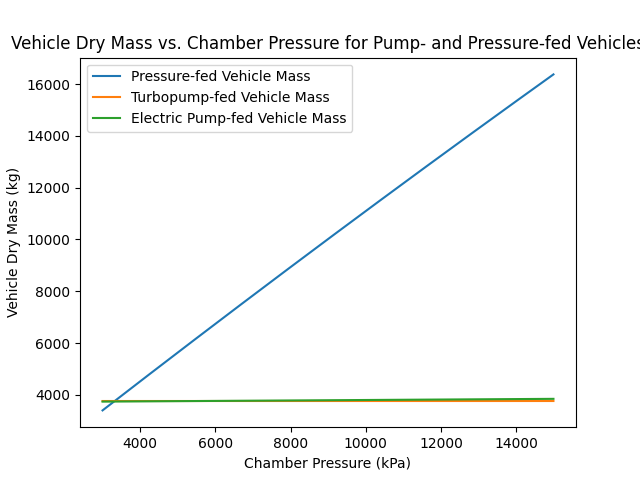
\includegraphics[width=8cm]{Plots and Graphs/VehicleMass_V_Pc.png}
    \caption{Simplified Comparison of Vehicle Mass for Pressure-fed, Turbopump-fed, and Electric Pump-fed Vehicles}
\end{figure}

\begin{figure}[t]
    \centering
    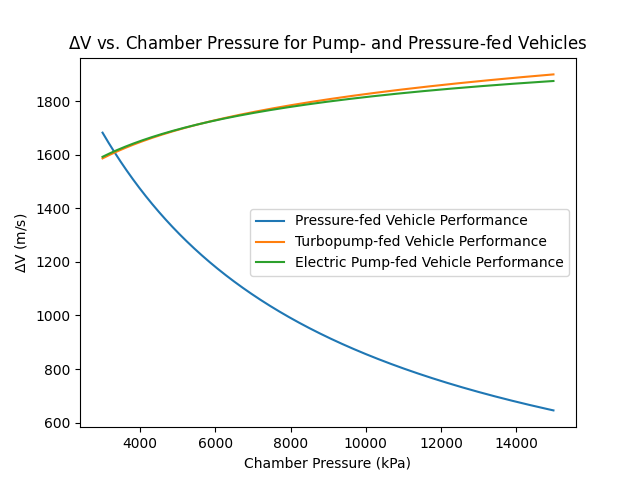
\includegraphics[width=8cm]{Plots and Graphs/deltaV_Pressure_V_Pump.png}
    \caption{Simplified $\Delta$V Comparison Against Chamber Pressure for Pressure-fed, Turbopump-fed, and Electric Pump-fed Vehicles}
\end{figure}

In a pump-fed vehicle, it is possible to achieve much higher performance by converting other, much more mass-efficient, types of energy into pressure energy. Most vehicles opt to use the same energy source that is being used to boost the rocket in the first place: chemical energy in the propellants. By taking a small amount of the overall chemical energy available in the propellant and dedicating it to increasing chamber pressure, a much higher overall engine performance can be obtained in a flight-worthy engine. In an open cycle, this chemical energy is only used to create pressure energy, and the propellant is dumped after it has accomplished this job. However, closed cycle engines are able to use this propellant to create thrust after it is used to generate the necessary pressures and flow rates. These categories of engine cycles, but especially closed cycle engines, require much greater complexity in engine operations and plumbing. This is because in addition to complex, custom components, turbopump-fed engines often must strike a delicate balance between various parts of the engine due to interconnected operations. This can especially complicate the startup procedure for the engine, as the pumps may rely on the combustion chamber to spool up. They also open up areas of potential risk to engine reliability and longevity, such as high-speed rotating shaft seals and combustion devices that may cause engine coking (gumming up) or pose a risk of component degradation due to high temperatures and pressures.

Electric pump-fed engines are also able to achieve high chamber pressures without the need for high pressure tanks. However, they eliminate much of the complexity introduced by turbopumps by simply powering the pumps using an electric motor or motors. This removes many components, such as turbines and gas generators/preburners. However, this also changes the energy source that is being tapped to generated the pressure energy and flow needed to run the engine. Rather than using chemical energy in the propellants, the chemical energy in a battery is used instead. This adds an additional energy source not needed for thrust generation that must be included on the vehicle. Because higher chamber pressure increases the power required by the pumps, this also necessitates a larger battery that can deliver this power and increases the overall mass of the vehicle. This is shown in Figure 5, which shows the steady increase in electric pump-fed vehicle mass as chamber pressure increases, while the turbopump-fed vehicle remains approximately the same mass. This is estimated using both the energy and power required by the pumps for a given chamber pressure and using energy and power density (Wh/kg and W/kg) values achievable by today's batteries. These values are calculated for the same vehicle with 2.2 metric tons of propellants held in 2195-T8 aluminum-lithium alloy tanks, the same that is used in the tanks of the Falcon 9. This analysis assumes that the power density of the turbopump and associated combustors is roughly the same as that of the electric motors used in the electric pump-fed engine, so the masses are equal for a given engine. This appears to be a reasonable assumption with both of these pieces of hardware estimated at around 10 kW/kg. 

As can be seen in Figure 6, this means that at very high chamber pressures, electric pump-fed engines lose some of the performance gained to battery mass.  The turbopump-fed vehicle continues to achieve appreciable $\Delta $V gains as chamber pressures are increased, while electric pump-fed vehicles effectively reach a performance limit. If we look closer at these relationships, however, it becomes clear that electric pump-fed engines can achieve much of the performance gains of turbopumps for  small-scale, low-to-medium performance vehicles. Up to chamber pressures of 5000 kPa, or 725 psi, the performance difference between the engines is only 3-4\%, showing that electric pump-fed engines can reach performance levels very near to turbopump-fed engines.

If we were to scale up the vehicles in this comparison, the performance differences would become larger. The reason for this is the square-cube law, which dictates that because tank mass grows with the square of vehicle size and propellant volume grows with the cube of vehicle size, the ratio of wet to dry mass increases as vehicles are scaled up. Said in another way, larger rockets are able to hold more propellant in proportionally lighter tanks. Because of this relationship and because pump power requirements scale proportionally with mass flow rate of propellant, this means that a larger electric pump-fed vehicle's battery will increase its dry mass by a greater proportion than a smaller electric pump-fed vehicle, which also increases the performance penalty of this extra mass. The maximum power that electric motors are able to deliver and the mass of the motors is also a bottleneck that will affect the maximum size of vehicle that electric pump-fed engines can realistically power. However, the threshold past which this performance penalty from battery mass is too large to be tenable and electric motors cannot provide the necessary power is somewhere between the sizes of a small and medium-lift orbital launch vehicles. Which means that I am confident in saying that this isn't likely to be an issue for most hobbyists and student teams in the near-term (if this does become a problem for you, you are doing something right). This makes electric pump-fed engines a very favorable choice for small vehicles like those likely to be built by a hobbyist or student team, especially because most vehicles of this type would never have been designed for chamber pressures high enough that the performance limits of electric pump-fed engines become significant. In summary, with electric pump-fed engines, it is possible to achieve very good performance while eliminating a huge portion of the design, manufacturing, and operational complexity.

\subsubsection{Existing Electric Pump-fed Vehicles and Engines}

This also explains why electric pump-fed engines have been used for many of the small launch vehicles that have been developed in recent years. The Rutherford engine that powers Rocket Lab's Electron is a high-performance kerosene-LOX dual-shaft electric pump-fed engine and power one of the most dependable workhorse rockets flying today. It is also one of the only engines to be recovered and refired following an orbital flight. This is also indicative of the reusability benefits of this kind of engine, as it eliminates many of the sources of wear that engines experience. Some hobbyists have also delved into electric pump-fed cycles, including some successful firings of partially pump-fed engines, one of which is pictured below. This has been a rare occurrence, however, and one of the goals of this document is to help more hobbyists and students get a start with this cycle.

\begin{figure}[]
    \centering
    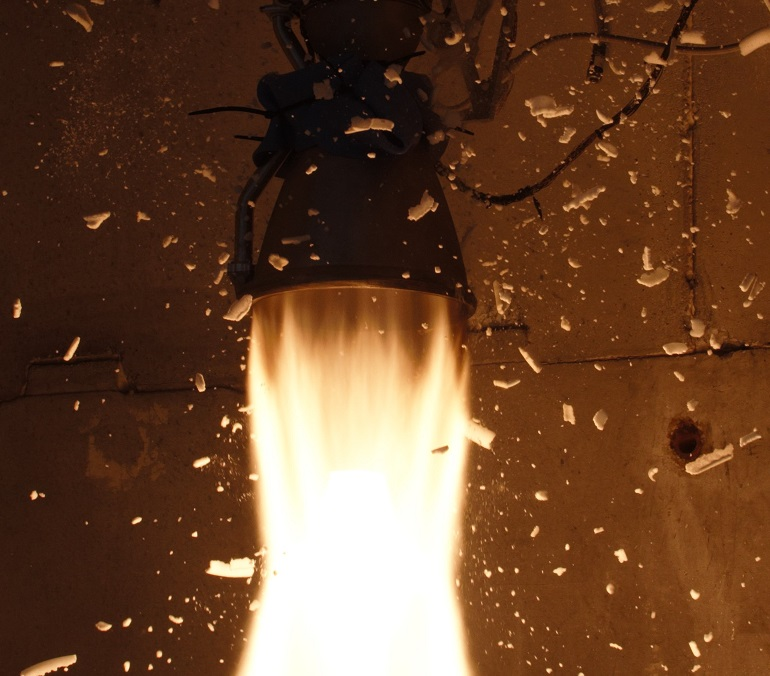
\includegraphics[width=8cm]{Images/Rutherford-Ignition3.jpg}
    \caption{Rocket Lab's Rutherford is Fired After Powering an Electron to Orbit}
\end{figure}

\begin{figure}[]
    \centering
    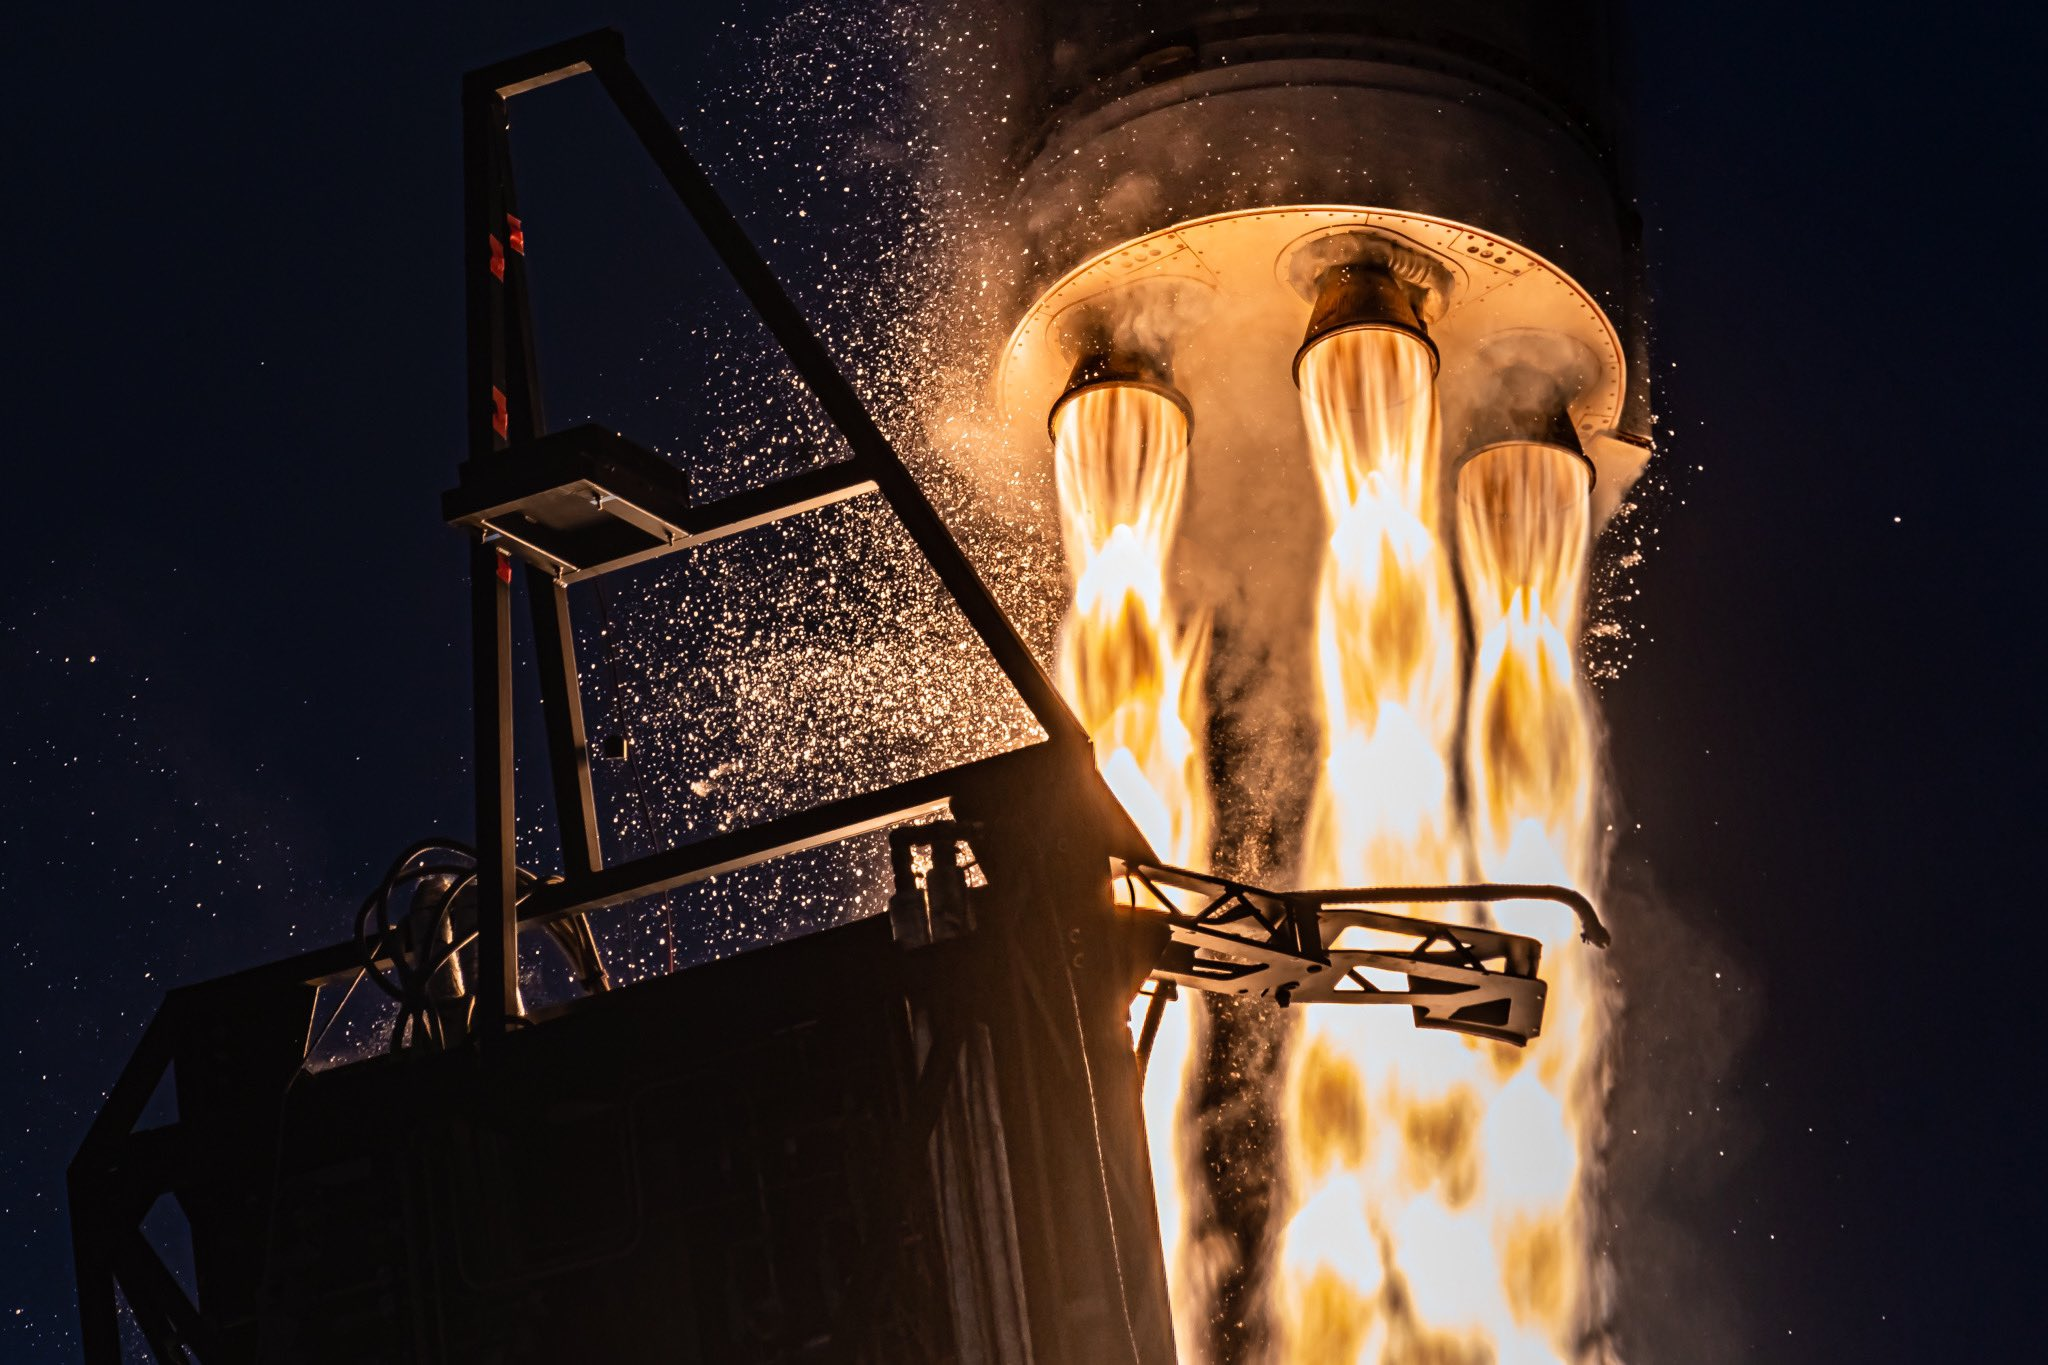
\includegraphics[width=10cm]{Images/AstraLaunch.jpg}
    \caption{Five Delphin Engines Power Astra's Rocket 3.2}
\end{figure}

\begin{figure}[t]
    \centering
    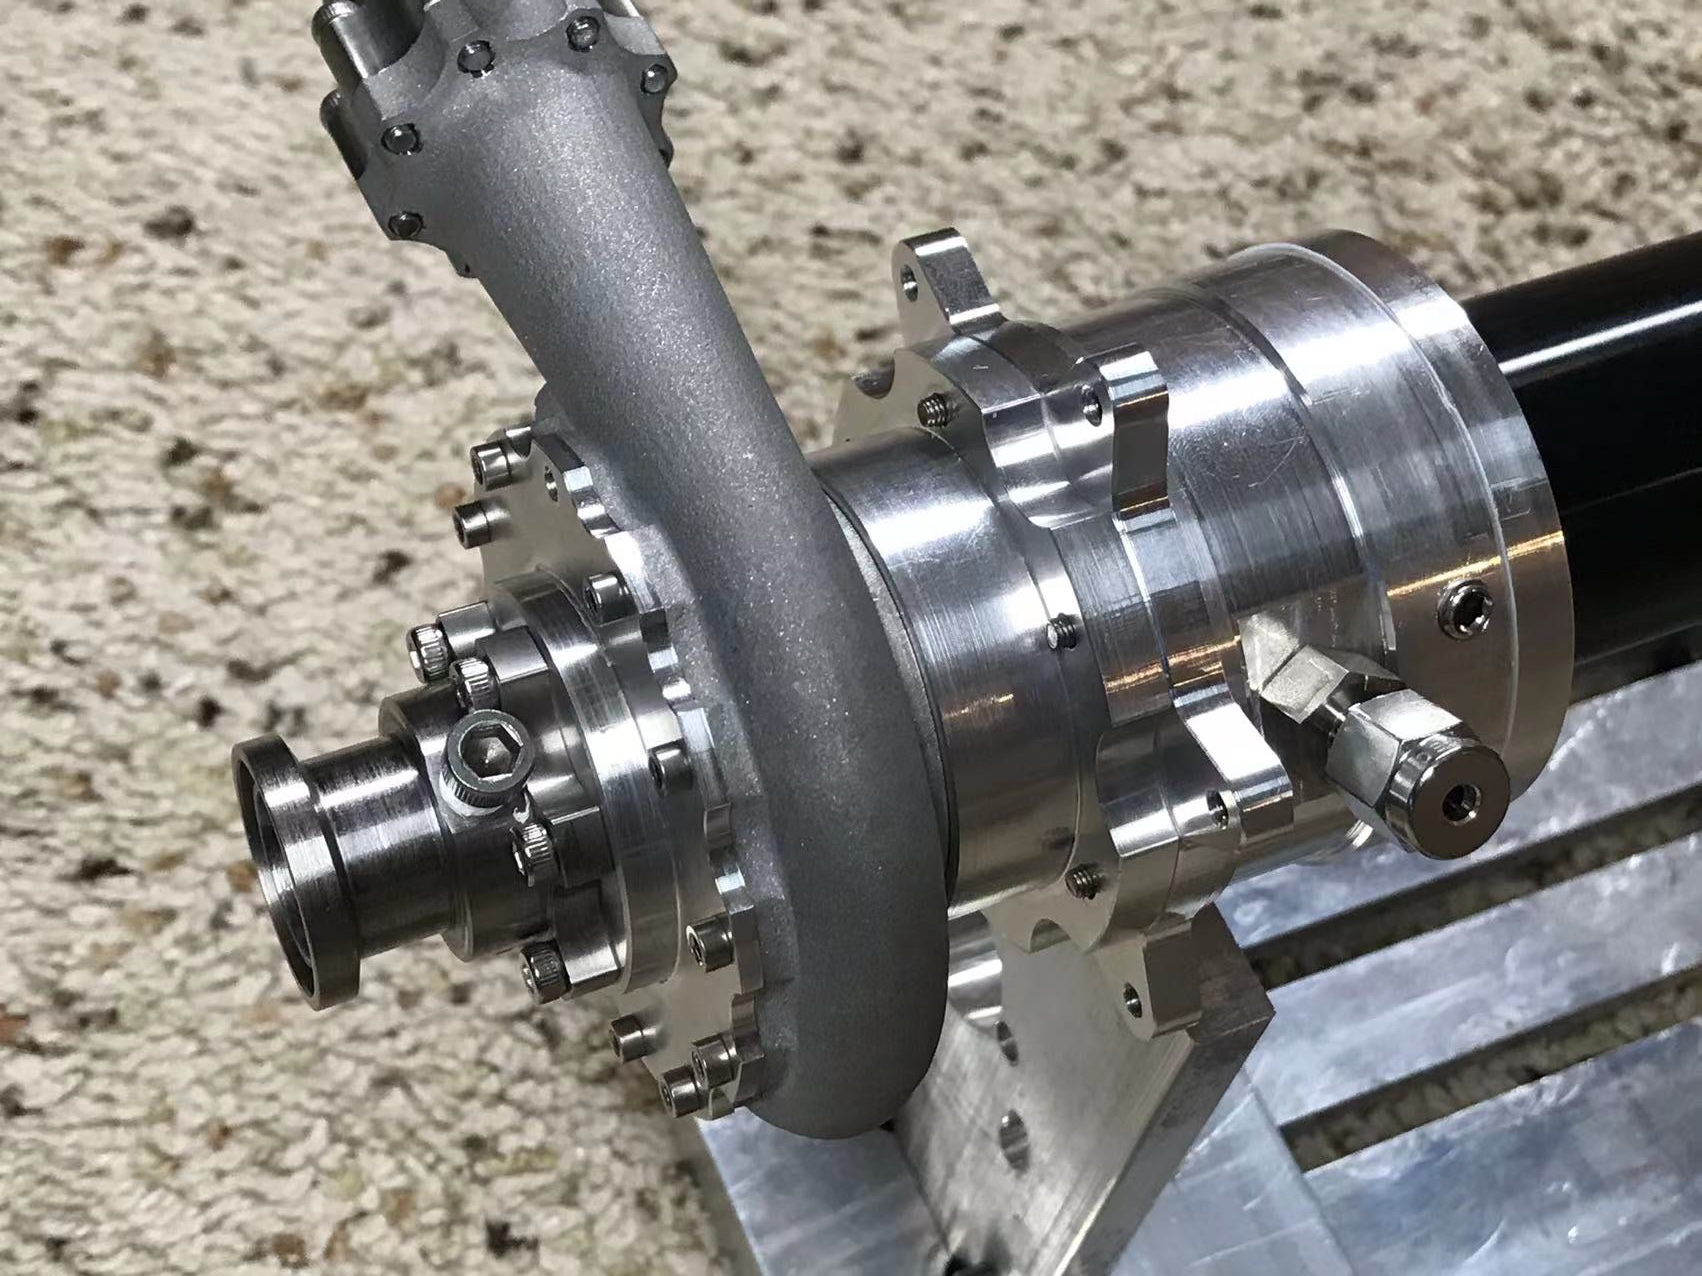
\includegraphics[width=10cm]{Images/Pump_LOX_reddit.jpeg}
    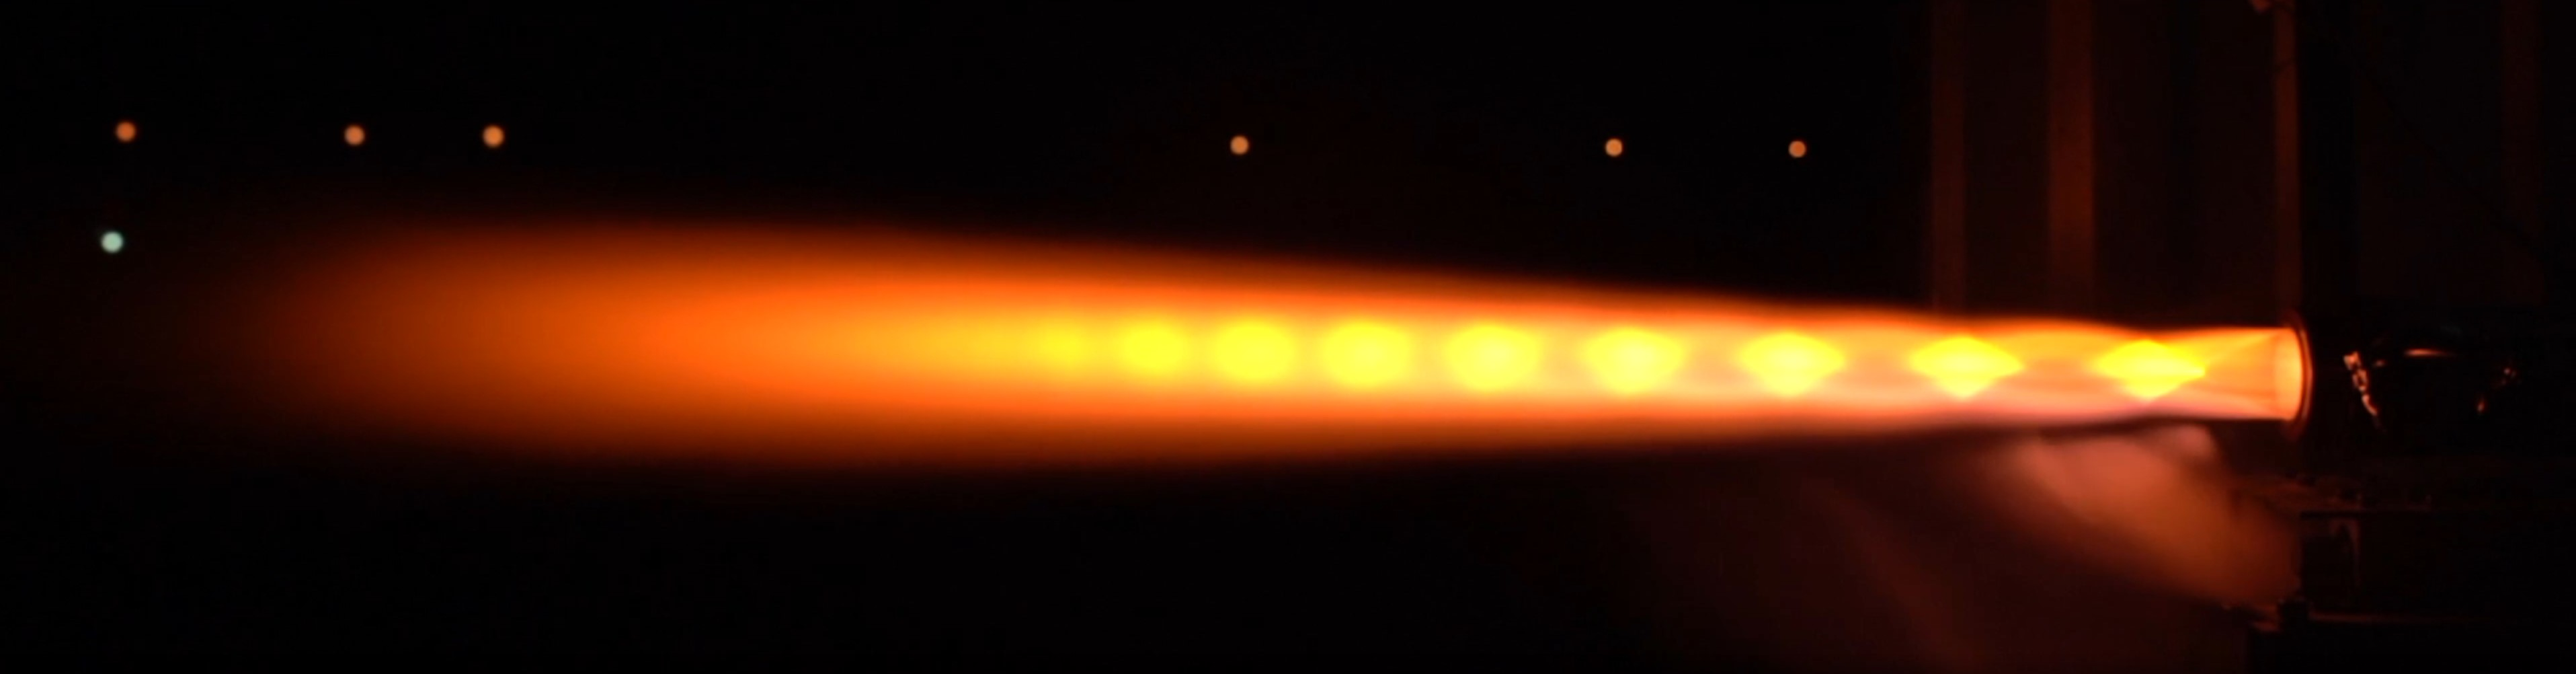
\includegraphics[width=10cm]{Images/ElectricPumpFedReddit.jpg}
    \caption{LOX Pump Assembly and Test Firing of Akarin's LOX and Ethanol Partially Electric Pump-fed Engine}
\end{figure}


\newpage

\subsection{Target Performance Metrics}

\begin{tabular}{|c|c|}

\hline

Engine Metric & Target Design Value \\

\hline

Maximum Thrust (kN) & 2 \\
Mass Flow Rate, LOX (kg/s) & 0.54921 \\
Mass Flow Rate, Kerosene (kg/s) & 0.24964 \\
Total Mass Flow Rate (kg/s) & 0.79885 \\
Chamber Pressure (psi) & 400 \\
Total Pump Required Power  (kW), $\eta$ = 100\% & 2.65 \\
Total Pump Required Power (kW) & 5 \\
Pump Efficiency (\%) & 53 \\
Maximum Firing Duration (s) & 60 \\
Mixture Ratio, O/F & 2.2 \\
Throttling Range (\%) & 70-100 \\
Throttling Range (kN)& 1.4-2 \\
Sea Level Specifc Impulse (s) & 254.5 \\
Expansion Ratio & 4.67 \\

\hline

\end{tabular}

\subsection{Turbomachinery Experience}
\subsection{Design of Key Engine Components}
\subsection{Flight-like Architecture}
\subsection{Rapid Testing Capabilities}
\subsection{Safety Objectives}
Lack of need for high-pressure tanks (at least non-GSE high-pressure tanks) when personnel are present at the pad

\section{Engine Architecture Overview}
\subsection{Propellants}
\subsection{Tanks}
\subsection{Valves}
\subsection{Flowmeters}
\subsection{Avionics and Sensing}
\subsubsection{Engine Controller}
\subsubsection{Pressure Transducers}
\subsubsection{Thermocouples}
\subsubsection{Communication}
\subsubsection{Power System}
\subsubsection{Load Cell}
\subsection{Torch Igniter}
\subsection{Fuel Pump}
\subsection{Oxidizer Pump}
\subsection{Injector}
\subsection{Thrust Chamber}

\section{Engine Firing Procedure}
\subsection{Nominal Firing Procedure}
\subsection{Contingency Scenarios}
\subsection{Engine Control Interface}
\subsection{Safety Measures}

\newpage

\section{Strata Development and Testing Roadmap}
\subsection{Test Program Overview}
\subsubsection{Test Program Gantt Chart}
\subsection{Tank Proof Testing}
\subsection{Pump Flow Testing}
\subsubsection{Pump Flow Test Setup}
\subsection{Torch Igniter Testing}
\subsubsection{Torch Igniter Test Setup}
\subsection{Injector Testing}

\newpage

\section{Notional VTVL Vehicle Design}
\subsection{Vehicle Architecture and Performance Metrics}

\begin{tabular}{|c|c|}

\hline

Vehicle Component & Estimated Component Mass (kg) \\

\hline

LOX & 49.5 \\
Kerosene & 22.5 \\
Valves & 45 \\
Tanks & 14 \\
Landing Legs & 4.5 \\
Piping, Fittings, etc & 10 \\
Pumps and Motors & 3 \\
Battery & 0.8 \\
Thrust Chamber and Injector & 7.5 \\

\hline

Total & 156.8 \\

\hline

\end{tabular}

\subsection{Vehicle Use Case}

\section{Primary Remaining Design Questions}

\section{Long-term Roadmap}
\subsection{Advanced Capabilities}
\subsection{Next-generation Electric Pump-fed Engine}
\subsubsection{Potential Performance Metrics}
What are the limits of performance for an electric pump-fed engine?

\subsection{Future Vehicles}
High altitude (karman line) rocket and high-speed/high-altitude hopper based on scaled up version of engine an upsized tanks made in the same way

\subsubsection{High Altitude Hopper}
Structural analysis to make sure the rocket can make it through max dynamic pressure
\subsection{More Advanced Engine Cycles}
\end{document}